%!TEX root = ../main.tex
The final version of the application runtime will be heavily dependent on the Programming Framework, whose model has been defined in~\cite{D7.2}. The current prototype has been developed with the following aims: 
% has been created before this effort has three goals:
\begin{itemize}
	\item To identify what the runtime should expect from a generic application;
    \item To define a first high level API to be provided to application developers;
	\item To test the interaction of the platform with the different components.
\end{itemize}

At the moment the platform mainly consists of a runtime allowing a Smart Society application to manage the submission of tasks by the user application. The platform provides also some library (against which the application is compiled) to operate with the current components (SmartCom, Orchestration Manager, Peer Manager). The code is in a private repository at \url{https://gitlab.com/smartsociety/appruntime}.

A Smart Society Application has its own identifier, generated during the registration phase. At the moment the application code is written by a developer directly in Java; in the final version of the platform the code will be generated dynamically through the programming framework. %Each time a task is submitted to the application a new application instance is created, each instance with its own state.

\subsection{Runtime}
Each application is expected to run in its own process by the SmartSociety runtime. The application will be provided by runtime with a SmartCom and a Orchestrator instances. In order to interact with external entities (such as peers or user applications), the runtime exposes three endpoints:

\begin{itemize}
\item {\bf POST:/task/:applicationId/} To submit tasks, the runtime will ask the application to create an \textit{instance initializer} that will take care of the setup phase of the task. The application is expected to carry out all the operation that can be performed before interacting with the peers. The posted data is domain--dependent, and it will be serialized and managed by the application at the moment of instance creation. The runtime associated to the instance (hence the task) creates an identifier that is returned as response for further usage.

\item {\bf GET:/task/:applicationId/} This endpoint is used to query the status of one or multiple tasks. Query parameters can be used to specify a filter on the tasks of interest. 
%all or part of the tasks of the application, query parameters can be used in the query and they will be managed by the application that might filter which tasks to show based non them. Note that t
The status format for each task is just required to be a valid json node (either a text or more complex structures) and it is completely domain--dependent. %, in fact the SmartSociety application can send whatever information the user application requires.

\item {\bf GET:/task/:applicationId/:taskId} Used to retrieve the status of a specific task. As for the previous point both query parameters and the response are domain--dependent.

\item {\bf POST:/message/:applicationId/} Used by the peer applications to communicate back with the application. To use this endpoint the application must have previously contacted the peer with a message containing a given conversation identifier. Such identifier is used then by the runtime to dispatch the message to the correct application instance. The content of the message is then handled by the task runner instance that changes its state according to the information received.
\end{itemize}

In v.2.0 of the platform, the application developer is expected to provide certain functionalities. This includes methods for:
\begin{itemize}
 	\item Creating a new task runner that will take care of setting up and carry out the task submitted to the application;
 	\item Retrieve the active task runners according to some query parameters, this will be used by the query endpoint.
\end{itemize}
The task runner is the instance of an application-specific class, which implements a simple interface allowing the runtime to start the execution and to ask for its status.


\subsection{Component Library}
The component library allows the application development to be abstracted from the actual implementation of the components.
Component wrappers provide a simple interface to the component integrated with the runtime, so that the developer will be shielded by minor changes in components. %, and finally testing will be easier as well.

In this section we briefly describe the functionality % give some example of functionalities 
provided by the component library. % divided by component.
\subsubsection{SmartCom}
The developer does not need to interact directly with \mdl: 
a method is provided for sending a message to a given collective, the programmer is required to provide a specific handler for handling answers to the message. The runtime will take care of receiving answers through the specific REST endpoint 
%(using an ad-hoc) 
and by using the conversation ID route the answer to the correct handler. The platform provides also an adapter for sending out Android notifications or for contacting peers trough a REST endpoint. Other supported adapters (Dropbox, Email, ...) can be easily added. 
%and adding them is straightforward.

\subsubsection{Orchestration Manager}
When the application is launched %At the application start time 
an orchestration manager (OM) is also executed. Communication with the OM works trough a REST API (a generalized version of the one presented in~\cite{D6.2}). % but this part is hidden to the developer, 
The library makes easy for the developer to make the following requests:
\begin{itemize}
	\item Submit a task request for composition;
	\item Retrieve a specific task request or task;
	\item Wait for a negotiable task;
	\item Accept a task on behalf of a peer;
	\item Perform a trivial negotiation with explicit agreement; 
	\item Wait for an agreed task.
\end{itemize}

Because of limitations of the current implementation of the PM the composition consists in retrieving all the peer registered to the application; this query is %, such a query is 
performed directly by the OM.

\subsubsection{Peer Manager}
The library allows the easy creation of a collective given a collection of peers. The identifier of the collective is the only thing needed by SmartCom to carry out communications transparently to the developer.

\subsubsection{Provenance}
The runtime provides easy methods for logging on the provenance store the generic (i..e, independent from the application domain) part of the provenance graph. % indipendent from the application domain.
Some helper function is provided for binding specific data whose model cannot be known a priori.
The communication with provenance store (happening through a REST API) is hidden to the developer by the library.

\subsection{Monitoring Framework}
%\todo{In the repository there is nothing like that}
The monitoring framework is responsible for the monitoring of the overall SmartSociety platform and components. It acts as a central collection point for any information which is considered important to ensure the proper functioning of the platform. More details are reported in App.~\ref{app:monitoring}.

% More in detail, it allows to:
% \begin{itemize}
% \item dynamically collect any kind of monitoring information relevant to monitor the proper functioning pf the platform and its performance. Such information is permanently stored in a non-relational database and available at any time for inspecting specific platform behaviors.
% \item visualize such information in real-time by means of interactive dashboards, or query the collected data via dedicated APIs. In particular, through the Monitoring framework it is possible to create and configure specific visualizations starting from the data that has been collected. There can be multiple visualizations, each one geared towards a specific platform KPI or informative visualization.
% \end{itemize} 

% %first, it allows to permanently store the data that is collected from the various COMPOSE components. The information can then be explored over time in order to either analyse the performance of platform components, or identify the causes of a specific malfunctioning. 
% %Second, it allows to visualize both real-time, as well historical data. In particular, through the Monitoring dashboard it is possible to create and configure specific visualizations starting from the data that is collected. There can be multiple visualizations, each one geared towards a specific platform KPI or information.
% %The COMPOSE platform administrator is expected to be the key utilizer of the Monitoring Dashboard. The current implementation does not support different visualizations based on user role.
% The Monitoring Dashboard is based on the following architecture and components:


% \begin{figure}[!hbt]
% \centering
% 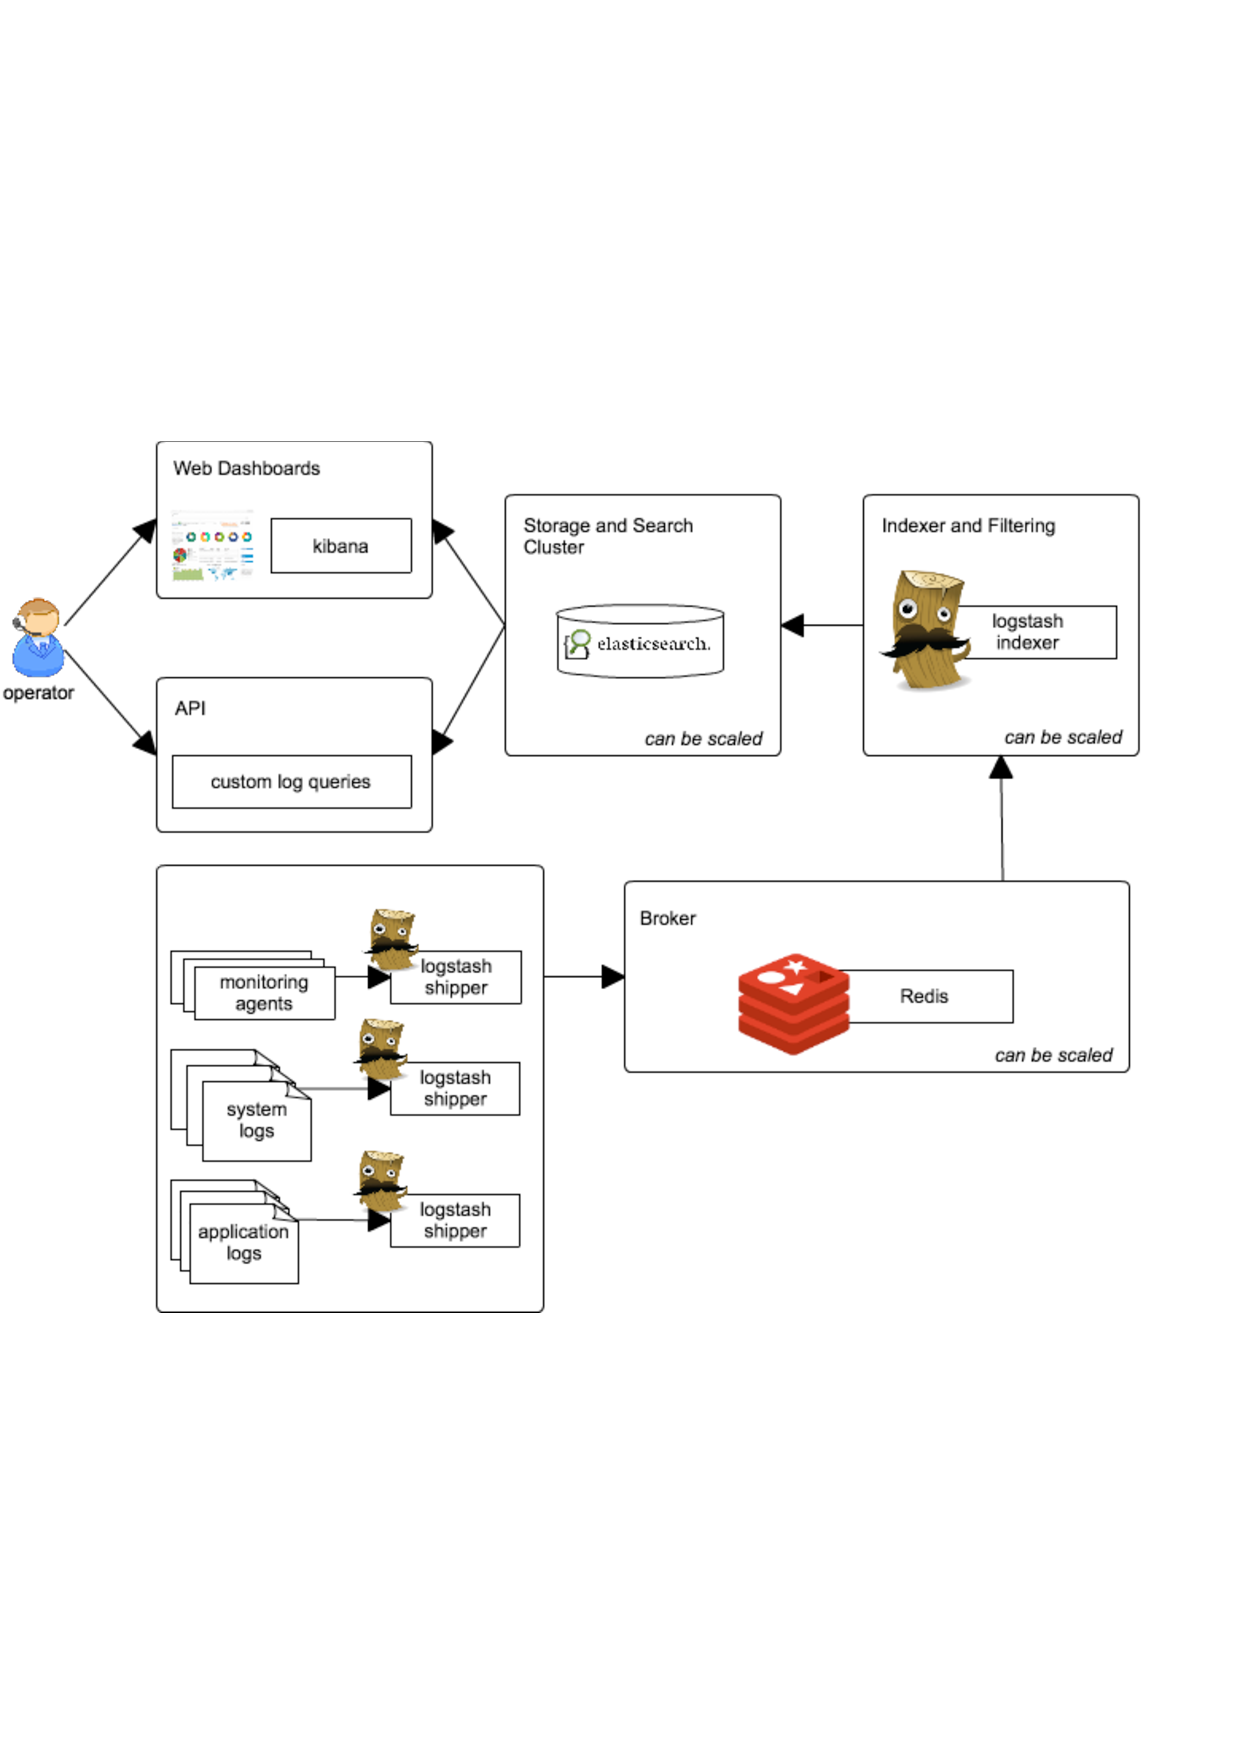
\includegraphics[width=0.8\textwidth]{figs/monitoring.pdf}
% \caption{Monitoring framework architecture.}
% \end{figure}

% The monitoring framework is based on Logstash (http://logstash.net/), which is a tool for managing events and logs. Logstash can be used to collect logs, parse them, and store them for later use (like, for search and visualization). Speaking of searching, Logstash comes with a web interface for searching and drilling into all of the logs collected over time.
% It is possible to define what information shall be permanently store and processed by the monitoring framework. In particular, it is possible to integrate:
% \begin{itemize}
% \item System logs: these logs correspond to logs, which are generated by the various system components such as, e.g., web servers, application servers. 
% \item Application logs: specific logs that are produced by applications, and require a constant integration for debugging and monitoring purposes.
% \item Monitoring information: any agent that can be configured to deliver data to the Logstash infrastructure.
% \end{itemize}

% In all three cases, a Logstash shipper is used to connect the specific source of data to Logstash. Specific shippers already exists for some widely use system components such as, e.g., web servers, databases, etc., while custom shippers can be created for specific cases. In the case of SmartSociety, we created a dedicated shipper to collect the events produced by the various platform components.\\
% The following component is a Redis Broker. This is an optional component that can be used in order to scale the system to large volumes of events and data. Based on Redis, data is indexed in order to prepare it for optimal searching and querying. Once the data is indexed, it is stored in an ElasticSearch cluster for storage and search. 
% Starting from the data stored in ElasticSearch, it is possible to build queries on scale to explore the collected data. We used Kibana (https://www.elastic.co/products/kibana) as the tool to create and visualize queries on the collected data. Kibana is fully integrated with ElastichSearch, and allows easily explore and give sense to large volumes of data.
% In addition, ElastichSearch provides APIs for querying and extracting the data stored in the platform. This can be helpful in the case aggregated views such as, e.g., monthly reports, are needed.
% The following Figure provides an example of dashboard created over Kibana. The metrics and specific charts can be configured dynamically by the administrator of the platform.

% \begin{figure}[!hbt]
% \centering
% 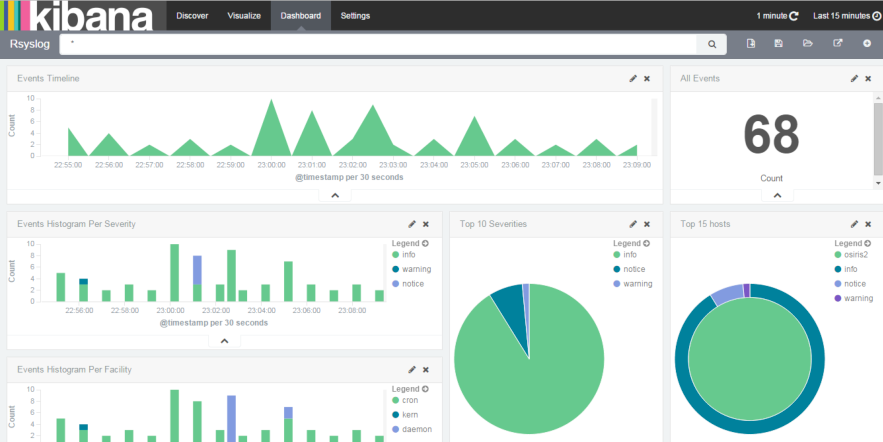
\includegraphics[width=0.8\textwidth]{figs/kibana.pdf}
% \caption{Example of the monitoring framework web interface.}
% \end{figure}


\subsection{Expected evolution}

In the future version of the platform each application and its runtime will be containerized. A service for routing the requests from general endpoints to the right application runtime will be included.

The way the runtime will evolve and its interaction with applications are highly dependent on the outcome of the programming model and programming framework specification efforts currently ongoing within WP7.